\documentclass{standalone}

\ifstandalone
	\usepackage{amsmath}
	\usepackage{pgfplots}
\fi


\begin{document}
	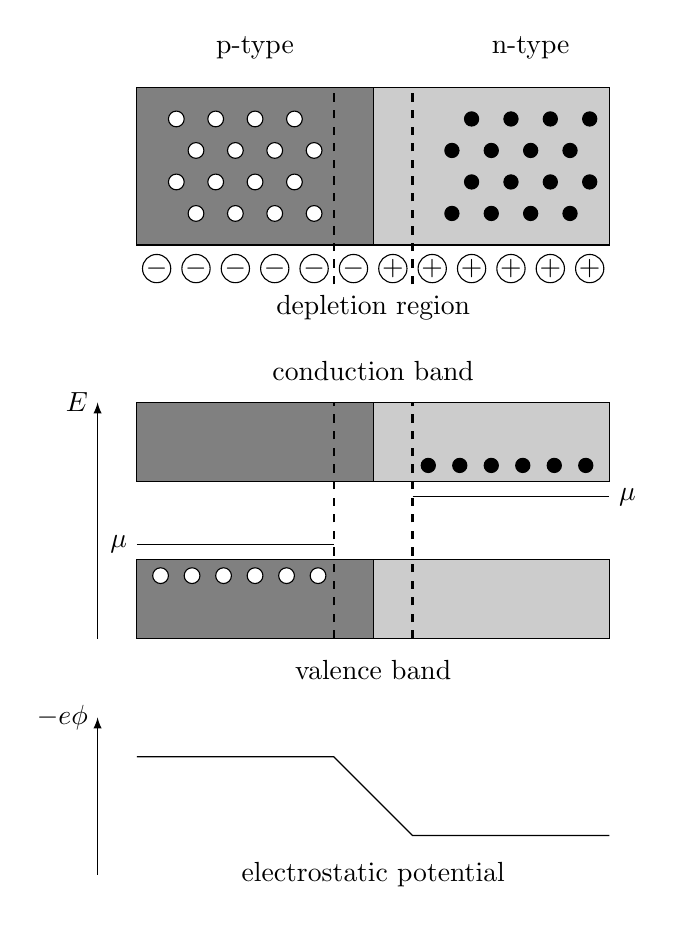
\begin{tikzpicture}
		\draw (1.5, 2.5) node {p-type};
		\draw (5, 2.5) node {n-type};
		\filldraw[draw=black, fill=gray] (0, 0) rectangle (3, 2);
		\filldraw[draw=black, fill=gray!40] (3, 0) rectangle (6, 2);
		\foreach \x in {1, ..., 4} {
			\filldraw[fill=white] (0.25+0.5*\x, 0.4) circle (.1);
			\filldraw[fill=white] (0.25+0.5*\x, 1.2) circle (.1);

			\filldraw[fill=black] (3.75+0.5*\x, 0.8) circle (.09);
			\filldraw[fill=black] (3.75+0.5*\x, 1.6) circle (.09);
		}
		\foreach \x in {1, ..., 4} {
			\filldraw[fill=white] (0.5*\x, 0.8) circle (.1);
			\filldraw[fill=white] (0.5*\x, 1.6) circle (.1);
			
			\filldraw[fill=black] (3.5+0.5*\x, 0.4) circle (.09);
			\filldraw[fill=black] (3.5+0.5*\x, 1.2) circle (.09);
		}
		\foreach \x in {0, ..., 5} {
			\draw (0.25+0.5*\x, -0.3) node[circle, draw=black, inner sep=0]{$-$};
			\draw (3.25+0.5*\x, -0.3) node[circle, draw=black, inner sep=0]{$+$};
		}
		\draw[dashed, line width=.8] (2.5, -.5) -- +(0, 2.5) +(1, 0) -- +(1, 2.5) +(0.5, -0.3) node{depletion region};

		\draw[-latex] (-0.5, -5) -- (-0.5, -2) node[left]{$E$};
		\filldraw[draw=black, fill=gray] (0, -2) rectangle +(3, -1) +(0, -1.8) node[left]{$\mu$} -- +(2.5, -1.8) ++(0, -2) rectangle +(3, -1);
		\filldraw[draw=black, fill=gray!40] (3, -2) rectangle +(3, -1) +(0.5, -1.2) -- +(3, -1.2) node[right]{$\mu$} ++(0, -2) rectangle +(3, -1);
		\draw[dashed, line width=.8] (2.5, -5) -- +(0, 3) +(1, 0) -- +(1, 3) +(0.5, -0.3);
		\draw (3, -1.6) node{conduction band} +(0, -3.8) node{valence band};
		\foreach \x in {0, ..., 5} {
			\filldraw[fill=white] (0.3+0.4*\x, -4.2) circle (.10);
			\filldraw[fill=black] (3.7+0.4*\x, -2.8) circle (.09);
		}
		
		\draw[-latex] (-0.5, -8) -- (-0.5, -6) node[left]{$-e\phi$};
		\draw (0, -6.5) -- ++(2.5, 0) -- ++(1, -1) -- ++(2.5, 0);
		\draw (3, -8) node{electrostatic potential};
	\end{tikzpicture}
\end{document}
